\normalfont\documentclass[letterpaper,11pt]{article}
\usepackage{amsmath, amsfonts,amssymb,latexsym}
\usepackage{fullpage}
\usepackage{parskip}
\usepackage{flexisym}
\usepackage{indentfirst}
\usepackage{graphicx}
\usepackage{algorithm2e}
% \usepackage{algorithm}
\usepackage{algorithmicx}
% \usepackage{algpseudocode}
\usepackage{amsmath}
\begin{document}
\setlength{\parindent}{2ex}
\newcommand{\header}{
	\noindent \fbox{
	\begin{minipage}{6.4in}
	\medskip
	\textbf{CS 271 -  Introduction to Artificial Intelligence} \hfill \textbf{Fall 2016} \\[1mm]
	\begin{center}
		{\Large HomeWork 1} \\[3mm]
	\end{center}
	  Name: \itshape{Liangjian Chen} \\
	  \textnormal{ID}: \itshape{\#52006933} \hfill \today
	\medskip
	\end{minipage}}
}
\bigskip
\header

\SetAlgoLined
\SetKwProg{MyStruct}{Struct}{ contains}{end}
\begin{enumerate}
\item[Problem 1]\par
	\begin{enumerate}
	\item
		\begin{enumerate}
		\item The struct is defined as follow\par
			\begin{algorithm}[H]
				\MyStruct{State}{
					int $Four$, $Three$\;
				}
			\end{algorithm}
		\item Define a pair of number (a,b) represent $Three$ is a and $Four$ is b.
			There is 14 different states in whole state space. They are:\\ 
			(0,0),(3,0),(0,4),(0,3),(3,4),(3,1),(3,3)\\
			(0,1),(1,0),(1,4),(3,2),(2,4),(2,0),(0,2)\\
		\item
			goal state is all the state that Three = 1.	So goal test is checking whether Three is one.
		\item
			(1) operation T-3, $Three \gets 3$ \\
			(2) operation T-4, $Four \gets 4$ \\
			(3) operation D-3, $Three \gets 0$ \\
			(4) operation D-4, $Four \gets 0$ \\
			(5) operation P-34(poure Three to Four)\\
			if $4 - Four \le Three$ then $Three \gets Three + Four - 4, Four \gets 4$. \\else $Four \gets Four + Three, Three \gets 0$\\
			(6) operation P-43(poure Four to Three)\\
			if $3 - Three \le Four$ then $Four \gets Three + Four - 3, Three \gets 3$.\\ else $Three \gets Three+ Four,Four \gets 0$
		\end{enumerate}
		\newpage
	\item
		The graph is shown below.\par
		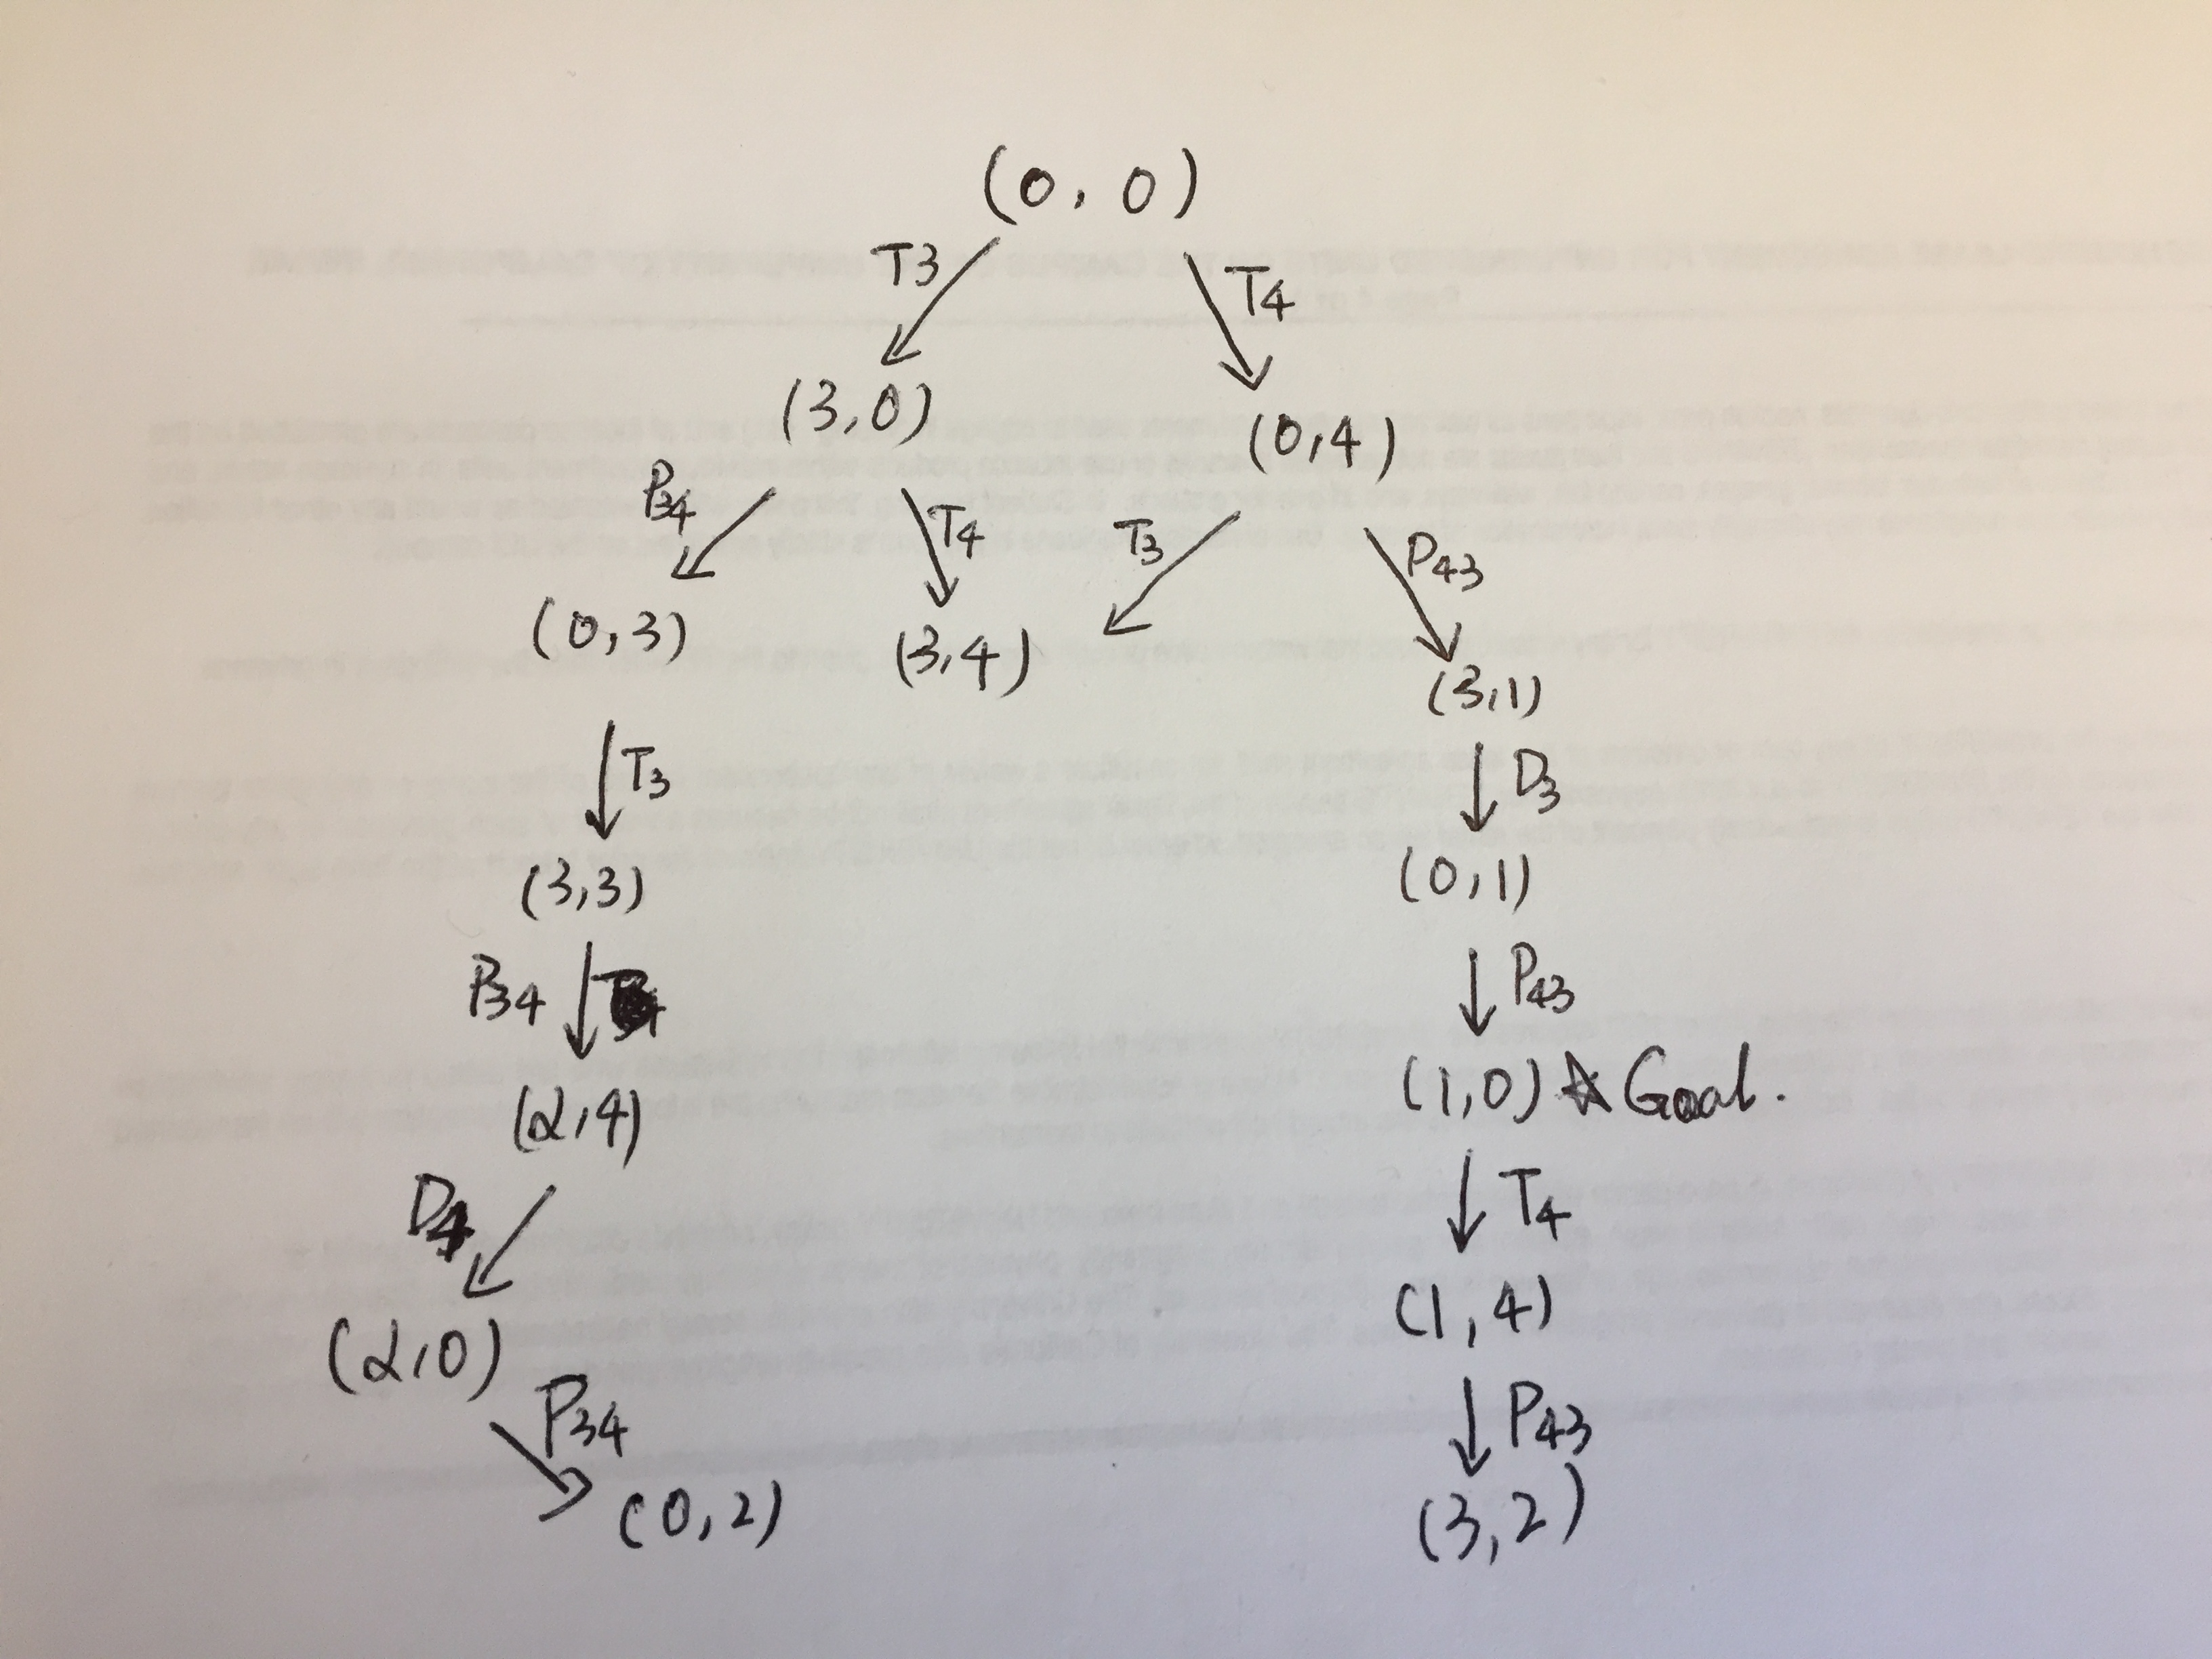
\includegraphics[height=10cm ,width=16cm]{1.JPG}
	\end{enumerate}
\item[Problem 2]\par
	\begin{enumerate}
		\item The struct is defined as follow\par
		\begin{algorithm}[H]
			\MyStruct{State}{
				int $M$, $C$\;
				char boat.
			}
		\end{algorithm}
			Here, M represent Missionary, C represent Cannibal.\\
			Let define the original side is side $A$, other side is side $B$. This State is how many Missionary and Cannibal on side $A$ and where is the ship. In this state space, there are $3 * 3 *2 = 18$ different state (including some illegal states).\\
			For short,Assume (x,y,z) means state(M,C,boat).\par
			So, initial state is (3,3,A), and goal state is (0,0,B);
		\item 
		Since there is 5 different choices, ship one or two people to another side.	\par	
		\begin{algorithm}[H]
			\eIf {$boat == A$}{
				\If {$M \geq 1 \textbf{ and } (M == 1 \textbf{ or } M - 1 \geq C)$}{					
					Go State(M - 1,C,"B")\;
				}
				\If {$M \geq 2 \textbf{ and } (M == 2 \textbf{ or } M - 2 \geq C)$}{
					Go State(M-2,C,"B")\;
				}
				\If {$C \geq1 \textbf{ and } (3 - M \geq 3 - C + 1 \textbf{ or } M == 3)$}{
					 Go State(M,C-1,"B")\;
				}
				\If {$C \geq2 \textbf{ and }(3 - M \geq 5 - C \textbf{ or } M == 3)$}{
					Go State(M,C-2,"B")\;
				}
				\If {$M \geq 1 \textbf{ and } C \geq 1$}{
					Go State(M-1,C-1,"B")\;
				}
			}{
				\If {$3 - M \geq 1 \textbf{ and } (3 - M == 1 \textbf{ or } 3 - M - 1 \geq C)$}{
					Go State(M + 1,C,"A")\;
				}
				\If {$3 - M \geq 2 \textbf{ and } (3 - M == 2 \textbf{ or } 3 - M - 2 \geq C$)}{
					Go State(M + 2,C,"A")\;
				}
				\If {$3 - C \geq 1 \textbf{ and } (M \geq C + 1 \textbf{ or } M == 0)$}{
					Go State(M,C + 1, "A")\;
				}
				\If {$3 - C \geq 2 \textbf{ and } (M \geq C + 2 \textbf{ or } M == 0)$}{
					Go State(M,C + 2, "A")\;
				}
				\If {$3 - M \geq 1 \textbf{ and } 3 - C \geq 1$}{
					Go State(M + 1,C + 1,"A")\;
				}
			}
		\end{algorithm}
		\item
		The graph is shown below.\par
		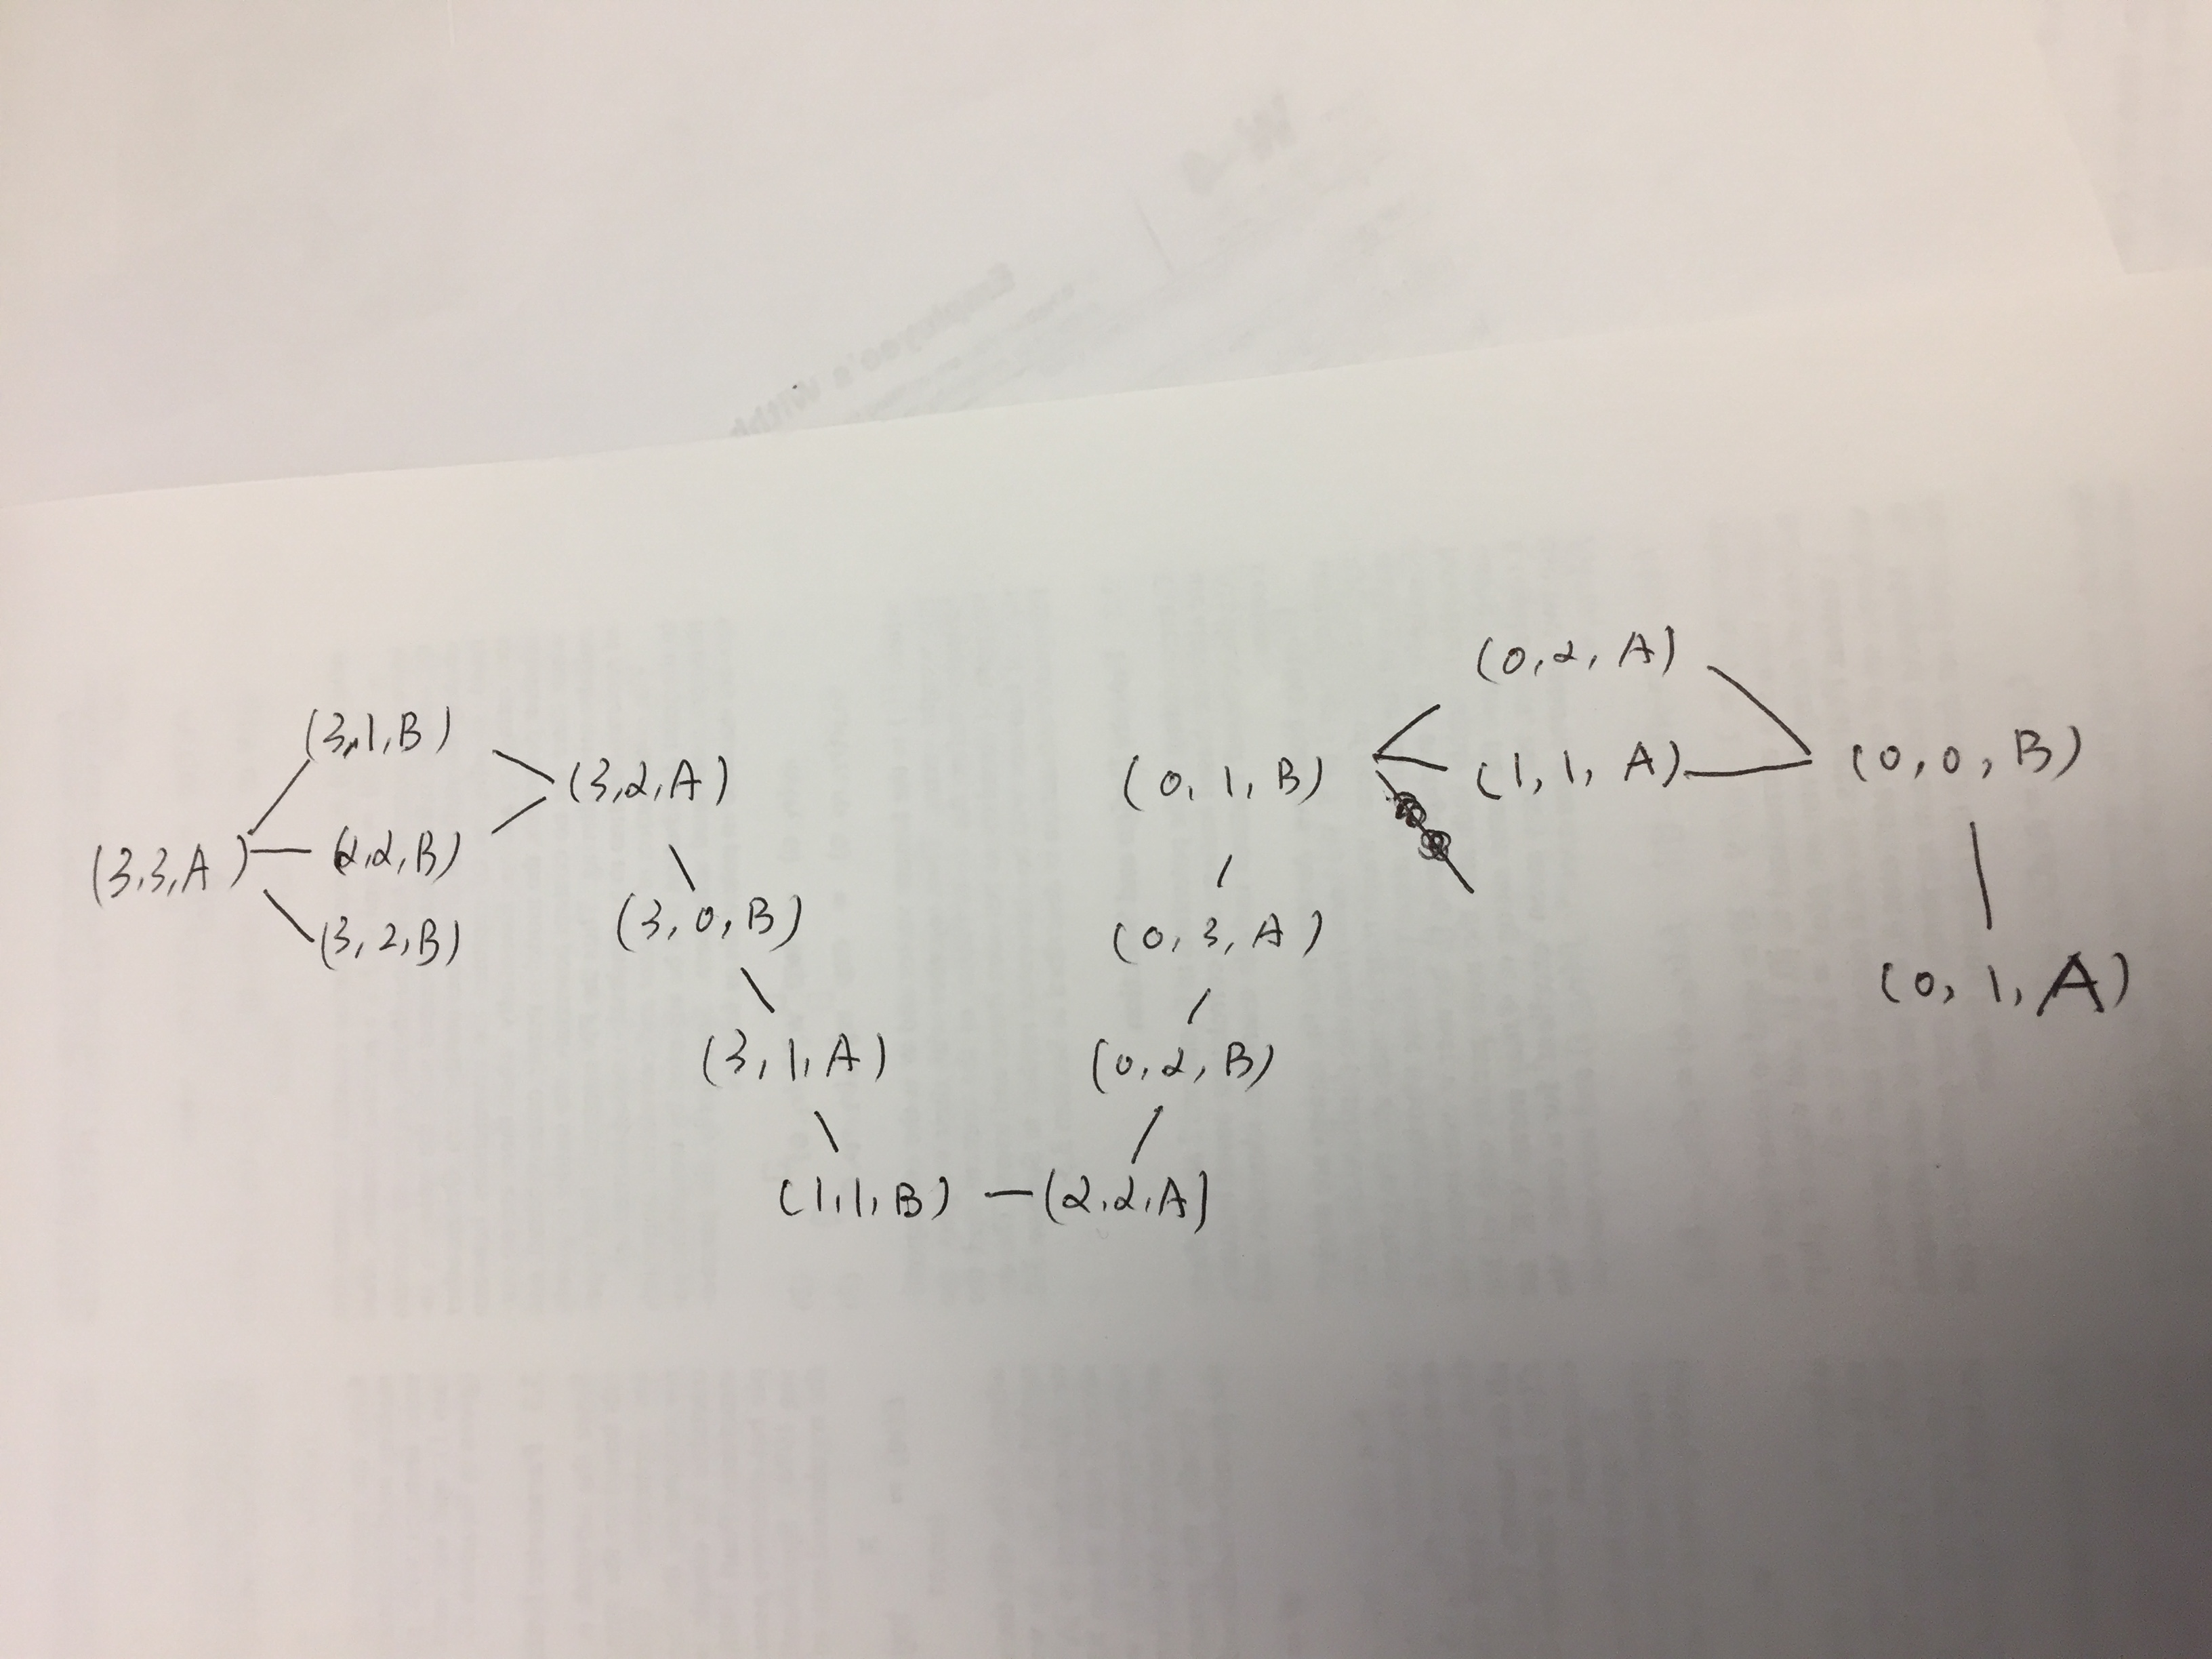
\includegraphics[height=12cm ,width=16cm]{2.JPG}

		\item
			Starting from the initial state, use the action set describe above, to find every possible next state. For every state which we have not visited yet, search it recursively until we find a goal state or there is no more available next state.
	\end{enumerate}

\item [Problem 3]\par
	\begin{enumerate}
		\item $S\to A\to B\to C\to F\to D\to E\to L\to M\to H\to I\to J\to K\to G$

		\item $S\to A\to D\to E\to J\to G$

		\item $S\to$\\
		$S\to A\to B\to C\to$\\
		$S\to A\to D\to E\to B\to F\to C\to H\to I\to$\\
		$S\to A\to D\to E\to J\to K\to L\to B\to F\to M\to C\to H\to I\to$\\
		$S\to A\to D\to E\to J\to G$
	\end{enumerate}
\item[Problem 4]\par
	\begin{enumerate}
		\item 
			$$\text{Max} = \sum_{i=0}^g{b^i} = \frac{b^{g+1} - 1}{b - 1} = O(b^g)$$\\
			$$\text{Min} = 1 + \sum_{i=0}^{g-1}{b^i} = 1 + \frac{b^{g} - 1}{b - 1} = O(b^{g-1})$$\\
		\item
			$$\text{Min} = g + 1 = O(g)$$\\
			$$\text{Max} = \sum_{i=0}^d{b^i} - \sum_{i=0}^{d-g}{b^i} + 1 = \frac{b^{d + 1} - 1}{b - 1} - \frac{b^{d-g + 1} - 1}{b - 1} + 1 = O(b^d)$$\\
		\item
			$$\text{Min} = g + 1 + \sum_{j=0}^{g-1}\sum_{i=0}^j{b^i} = \frac{b^{g+1} - b}{(b-1)^2} - \frac{g}{b-1} + g + 1 = O(b^{g-1})$$\\
			$$\text{Max} = \sum_{j=0}^{g}\sum_{i=0}^j{b^i} = \frac{b^{g+2} - b}{(b-1)^2} - \frac{g+1}{b-1} = O(b^g)$$\\
	\end{enumerate}
\item [Problem 5]\par
		For a graph $G(E,V)$,the number of comparison is equal to the number of edge $|E|$. Because degree is $b$ and depth is $d$, $|E| = \frac{b|V|}{2}$. Then larger the number of node is, larger the number comparison is. And know that there are at most $1 + \sum_{i=0}^{d-1}{b(b-1)^i} = O(b^d)$ nodes. Thus, the number of comparison is $O(b^d)$.\par
		Extra credit:\par
			Assume $f(b,d)$ is the maximum possible number of node in the graph.\\
			In this case, the number of comparison is $\sum_{i=0}^{f(b,d)}i = O(f(b,d)^2) = O(b^{2d})$



\end{enumerate}
\end{document}
